\documentclass{beamer}
\usepackage[export]{adjustbox}
\usepackage{comment}                % Comments...
\usepackage{graphicx}
\usepackage{wrapfig}
\graphicspath{ {/home/justinting/programming/jt-honours/images/} }
\usepackage[parfill]{parskip}       % Newline instead of indentation per paragraph
\usepackage[round]{natbib}
\usepackage{pgfpages}
\setbeameroption{show notes}
\setbeameroption{show notes on second screen=right}
\setbeamertemplate{background canvas}[vertical shading][bottom=white,top=structure.fg!35]
\setbeamertemplate{sidebar canvas left}[horizontal shading][left=white!40!black,right=black]
\beamertemplatenavigationsymbolsempty

\begin{document}

\begin{frame}
    \frametitle{Machine Learning in Benthic Habitat Mapping}
    \textbf{Justin Ting} | Honours Student

    \textbf{Simon O'Callaghan} | NICTA Researcher

    NICTA

    SIT

\end{frame}

%%%%%%%%%%%%%%%%%%%%%%%%%%%%%%%% INTRODUCTION %%%%%%%%%%%%%%%%%%%%%%%%%%%%%%%%
\begin{frame}
    \frametitle{Introduction}
    % \begin{wrapfigure}{1}{0.3\textwidth}
    \centering
    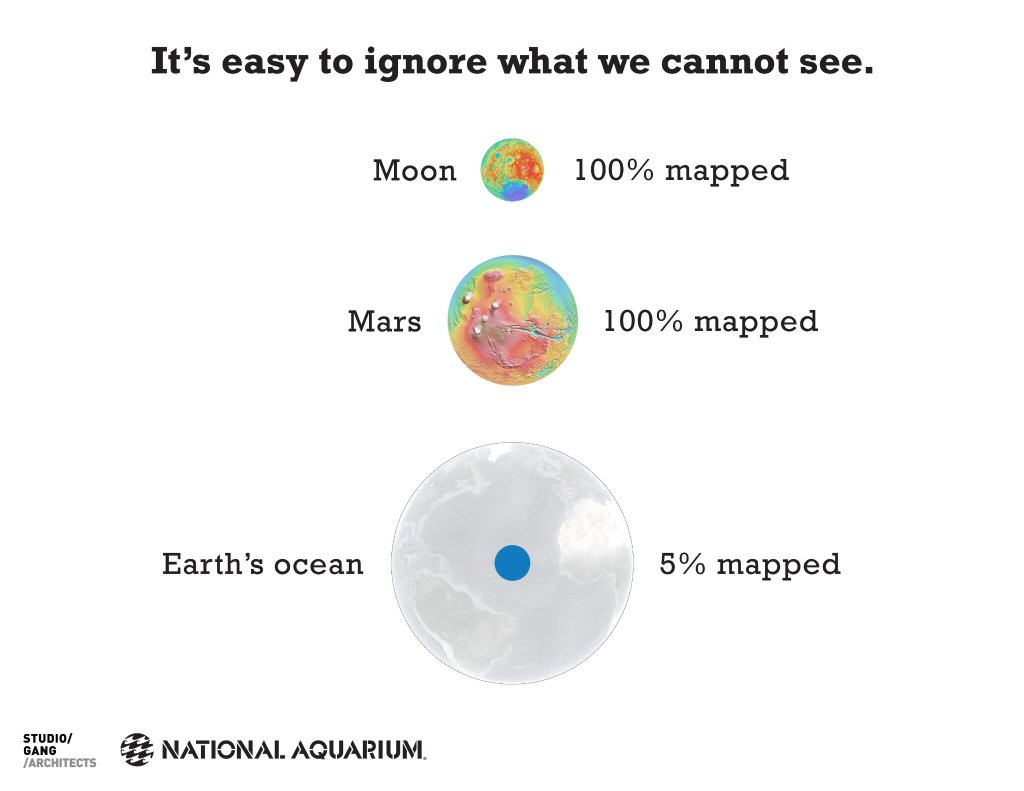
\includegraphics[scale=0.2,center]{oceans-mapped.jpg}\footnote{{\tiny Copley, J. (2016). » Mapping the deep, and the real story behind the “95\% unexplored” oceans. [online] Moocs.southampton.ac.uk.}}
    % \end{wrapfigure}
\end{frame}
\note{
    NOTE: These are the presenter notes that won't be seen by the audience during the presentation. Special software written for LaTeX-beamer slides will be used during the presentation to achieve this.

    0.75 minutes

    Less than 10\% of the Earth's oceans have been mapped to date - oceans that occupy 71\% of the Earth's surface. There a lot of reasons that we would want to increase this number - by better understanding the layout of the Earth's oceans, we can predict and project the state of its many ecosystems using limited data. This is crucial for conservation, as we can monitor how it is coping with changing environmental conditions, and subsequently take necessary action to preserve its state. 

\iffalse
    \begin{itemize}
        \item 0.5 minutes
        \item Why Benthic habiat mapping - we're interested in understand the layout of the ocean's habitats
        \item Benthic - ecological region at the lowest level of a body of water (benthos)
        \item Habitat mapping - based on a small amount of high resolution data, and a considerably larger amount of lower resolution data, a relationship is created to correlate the data in overlapping regions, which is then projected to the regions without the high resolution data to create a 'habitat map'
        \item Doing this is crucial for conservation, understanding the marine world, and how it is coping with changing environmental conditions
        \item The high resolution data is generally actual sediment samples or organism samples at the benthos
        \item Low resolution data is generally some sort of acoustic data representing basic properties of the seafloor
    \end{itemize}
\fi
}

\begin{frame}
    \frametitle{Introduction (cont.)}
    \begin{itemize}
        \item To map more of the world's oceans at a high resolution, we employ benthic habitat mapping techniques
        \item Combine sparse high resolution data with large(r) volumes of low resolution data
        \item Marine habitat mapping cuts across marine biology, geology, hydrography, oceanography, geophysics~\citep{cjbrown11}, along with machine learning
    \end{itemize}
\end{frame}
\note{

    The most prevalent way of doing this is using a method called benthic habitat mapping. The term 'benthic' refers to the ecological region at the lowest level of a body of water. Habitat mapping is the process of using a small amount of high resolution data and a considerably larger amount of lower resolution data, and modeling or creating a relationship with the data that overlaps in terms of the area which they represent. That relationship is then projected to the regions without the high resolution data, thus resulting in a habitat map.

The high resolution data is generally photos or videos of the seafloor, along with sediment or organism samples at the benthos, while the low resolution data is usually some form of acoustic data that can provide basic properties of the seafloor. This is done by firing off radio waves whose returning frequency are strength are measured, from which information such as depth, density (and hence material), roughness, slope, etc. can be extrapolated.

}

%%%%%%%%%%%%%%%%%%%%%%%%%%%%%%%% PROBLEM STATEMENT %%%%%%%%%%%%%%%%%%%%%%%%%%%%%%%%
\begin{frame}
    \frametitle{Problem Statement}
    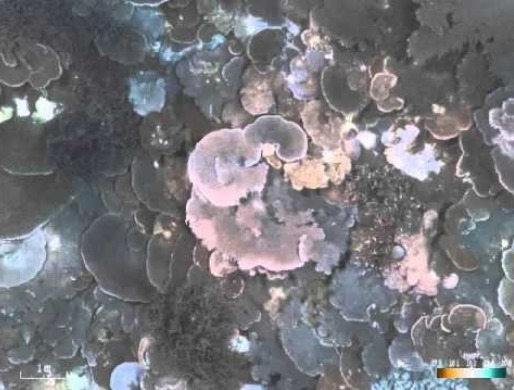
\includegraphics[scale=0.3,center]{some_marine_stuff.jpg}
    \begin{itemize}
        \item Much research in benthic habitat mapping generates deterministic maps using as-is machine learning techniques/implementations
        \item We need to be able to monitor marine habitats on a large scale to assess human impact over time to be able to make informed management decisions
    \end{itemize}
\end{frame}
\note{
    {\scriptsize
    1 minute

    A problem (although the same can be said of any machine learning) is that the assumed correlation between collectible data, which has been debated and contested across various studies, is debated and contested across various studies undertaken in benthic habitat mapping. It is arguably impossible to decisively confirm or deny these relationships without actually exploring a majority of the entire ocean - the expeditions for which would be prohibitively expensive. 

    In the absence of such confirmation, we want to both quantify the uncertainty of the maps generated and do so without assuming relationship between data features, so that appropriate decisions can be made, and even potentially gather more data regarding areas of low certainty, resulting in more focussed and efficient use of resources. Morever, using these probabilities, we want to be able to generate more accurate maps, with higher certainty, than was done in previous studies. 

    \iffalse
    \begin{itemize}
        \item 1 minute
        \item Weakness in benthic habitat mapping is the assumed correlation between collectible data, which has been debated and contested across various studies
        \item It is arguably impossible to decisively confirm or deny these relationships without actually exploring a majority of the entire oceans - expeditions whose cost are far too prohibitive
        \item In the absence of such confirmation, we want to quantify the certainty of the maps generated, so that appropriate decisions can be made, and potentially gather more data regarding areas with low certainty - more focused use of resources
        \item Use of 'vanilla' algorithms such as random forests in ~\citet{lucieer13}, ~\citet{seiler12}, ~\citet{hasan14}
    \end{itemize}
    \fi
    }
}

%%%%%%%%%%%%%%%%%%%%%%%%%%%%%%%% SOLUTION %%%%%%%%%%%%%%%%%%%%%%%%%%%%%%%%
\begin{frame}
    \frametitle{Solution - Overview}
    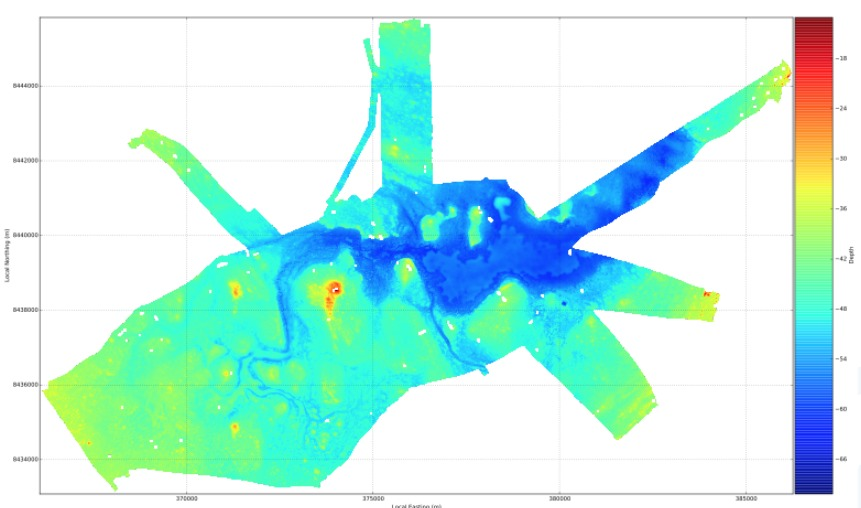
\includegraphics[scale=0.15,center]{scott_bathy.jpg}
    \begin{itemize}
        \item We will use Gaussian processes to make predictions on all the low resolution data, which provides a distribution of probable habitats for a given area
        \item 7 million bathymetry data points without matching high resolution data
        \item Probabilistic approach allows us to state certainty about a particular mapped area
        \item High resolution images were clustered into habitat classes using Variational Dirichlet Processes, an unsupervised method
    \end{itemize}
\end{frame}
\note {
    {
    To attempt to improve this problem, we use Gaussian processes for the classification process - and as a result, obtain a distribution of probable habitats for a given area rather than a deterministic result for a given space, and can thus state our certainty of a particular classification for an area of the benthos. Moreover, because the high resolution data used were images collected using automated vehicles that were then pre-clustered in ~\citet{steinberg11} using VDPs, the classifications themselves are represented as continuous probabilities.

    However, there is an inherent limitation in the use of Gaussian processes in that its computational complexity is $O(n^3)$ - meaning that for our relatively 'small' training dataset of 16,000, naive use of GPs are already computationally infeasible - let alone our unclassified dataset of 7 million for which we only have low resolution data.

    \iffalse
    \begin{itemize}
        \item 1 minute
        \item To encapsulate the uncertainty in the predictions we make regarding benthic habitats, we will use Gaussian processes to perform habitat classification
    \end{itemize}
    \fi
    }
}

\begin{frame}
    \frametitle{Solution - Overview}
    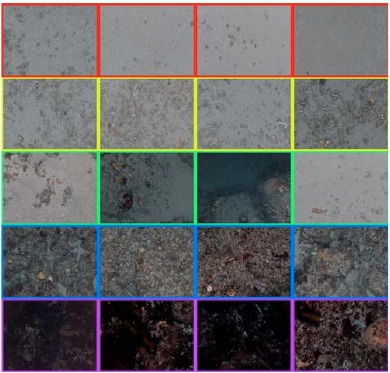
\includegraphics[scale=0.4,center]{clusters.jpg}

    ~\citet{bender12}
    \begin{itemize}
        \item The high resolution data that we used were images collected from autonomous underwater vehicles (AUVs), and already pre-clustered under another study by ~\citet{steinberg11}, using variational dirichlet processes (VDPs)
    \end{itemize}
    \note{
        The clusters here are an example of the unsupervised clustering of the high resolution images, using the same method that was used to cluster our data.
    }
\end{frame}

\begin{frame}
    \frametitle{Solution - Overview}
    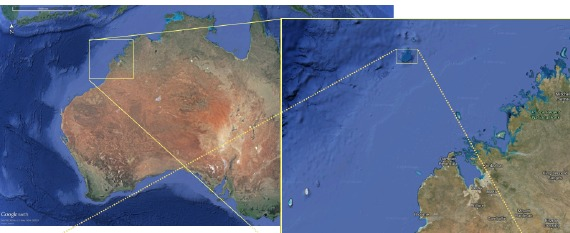
\includegraphics[scale=0.6,center]{scott_location.jpg}
\end{frame}
\note{
    The data was all collected from Scott Reef, a lagoon off the coast of Western Australia
}

%%%%%%%%%%%%%%%%%%%%%%%%%%%%%%%% SOLUTION - GPs %%%%%%%%%%%%%%%%%%%%%%%%%%%%%%%%
\begin{frame}
    \frametitle{Solution - Gaussian Processes (GPs), Sparse GPs}
    \begin{itemize}
        \item What are Gaussian Processes?
        \item Computational limitations with GPs
        \item Overcoming computational barriers using approximations
        \item Cooercing squashed GPs in classification to utilise studies in approximated sparse GP regression
        \item Expectation Propagation vs. Laplace method
    \end{itemize}
\end{frame}
\note {
    {\tiny
    To explain Gaussian processes in simple (and very brief) terms - first consider a single variable that fits a Gaussian distribution, commonly known as the bell curve, or normal distribution. If we generalise this single dimension to infinitely many, where any linear combination of components is normally distributed, then this is essentially a Gaussian Process.

    Compared to more commonly used supervised classification algorithms which require modeling around the chosen features, Gaussian processes instead look at the joint distribution across all features. However, they require a matrix inversion step with $O(n^3)$ complexity - this does not scale well beyond at most several thousand datapoints. To overcome this and be able to utilise as much of the available data as possible, we use approximation methods.

    While a number of studies have undertaken comparing approximating techniques in sparse GP regression, there are less similar studies for classification. The two are different because in the classification scenario, the function that is otherwise used in regression has to be passed through a squashing function to bound the results between (0, 1), resulting in a non-Gaussian distribution. A study by ~\cite{kuss05} found that Expectation Propagation was superior to the previously used Laplace's method. It is using Expectation Propagation that we will be able to use approximated sparse GP regression techniques and apply them to classification.
    }
    
    \iffalse
    \begin{itemize}
        \item 1.5 minutes
    \end{itemize}
    \fi
}

%%%%%%%%%%%%%%%%%%%%%%%%%%%%%%%% RESULTS 1 %%%%%%%%%%%%%%%%%%%%%%%%%%%%%%%%
\begin{frame}
    \frametitle{Results}

    \begin{itemize}
        \item Benchmarks using basic deterministic algorithms on the test dataset
        \item This first set of results is using 24 separate habitat classes as the labels.
        \item Two 'sets' of habitat classes were used - the original 24 labels, plus 5 aggregated labels
    \end{itemize}

    {\scriptsize
    24 Habitat classes

    \begin{tabular}{| l | l | l |}
        Algorithm           & F1 score & Accuracy \\\hline
        KNN (5)             & 0.33278 & 0.62459 \\
        Logistic Regression & 0.20285 & 0.682705 \\
        Random Forest       & 0.20283 & 0.68258 \\
        SVM                 & 0.20284 & 0.68270 \\
    \end{tabular}

    5 Aggregated habitat classes

    \begin{tabular}{| l | l | l |}
        Algorithm           & F1 score & Accuracy \\\hline
        KNN (5)             & 0.61347 & 0.749214 \\
        Logistic Regression & 0.50381 & 0.814503 \\
        Random Forest       & 0.50932 & 0.819253 \\
        SVM                 & 0.50290 & 0.818273 \\
    \end{tabular}
    }
\end{frame}
\note{
    {\scriptsize
    30 seconds

    Before looking at results of our Gaussian process (GP) classifier using varying sparse approximate GP methods, we want to obtain some basic 'benchmarks' by getting the F-score (average of precision and recall) and accuracy using some basic machine learning algorithms. The first table represents the original 24 granular classes, whereas the second one is using the 5 aggregated classes, which are basically a summarisation of the more specific 24, which was achieved in collaboration with an expert who grouped the original habitat classes together into similar clusters.
    
    The aggregated classes provide an obvious advantage in performance, due to the combination of similar habitats into clusters.

    \iffalse
    \begin{itemize}
        \item 15 seconds just highlighting results here
        \item a more coarse mapping of the habitats created in collaboration with an expert
        \item e.g. with labels 1-24, 1, 3, 5, 7 are condensed to one habitat, as they may be very similar visually, e.g. all sand with slight variations
        \item this brought the number of classes down to 5. The accuracy increases notably when the aggregation of visually matching habitat classes is performed.
        \item We would like to compare the results obtainable from use of Gaussian Processes in generating habitat maps to those of more naive methods. Note that measurements are taken by averaging over 10-fold cross validations.
        \item The accuracies don't break 20\%, and the f-scores, which are the average of the precision and recall, are considerably worse
        \item Results have improved considerably after aggregation - by a factor of 4-7 times for f-score, and 2-3 times for accuracy
    \end{itemize}
    \fi
    }
}

%%%%%%%%%%%%%%%%%%%%%%%%%%%%%%%% RESULTS 2 %%%%%%%%%%%%%%%%%%%%%%%%%%%%%%%%
\begin{frame}
    These final two set of results are using Gaussian processes with the granular and aggregated habitat classes, respectively, with different methods applied to minimise the original $O(n^3)$ computational complexity as much as possible. With the exception of the subset of data (SoD) benchmark, the rest are wrapped with Expectation Propagation

    {\scriptsize
    24 Habitat classes 

    \begin{tabular}{l | l | l}
        Approximation method    & F1 score & Accuracy \\\hline
        Subset of Data          & 0.72948 & 0.84106 \\
        SR                      & 0.79258 & 0.87151 \\
        PP                      & 0.81755 & 0.89162 \\
        FIC                     & 0.83291 & 0.91418
    \end{tabular}

    5 Aggregated habitat classes

    \begin{tabular}{l | l | l}
        Approximation method    & F1 score & Accuracy \\\hline
        Subset of Data          & 0.84281 & 0.91968 \\
        SR                      & 0.88954 & 0.93014 \\
        PP                      & 0.91758 & 0.95417 \\
        FIC                     & 0.92856 & 0.96281 
    \end{tabular}

    }

    {\tiny
    Key:\\
    SR - subset of regressors ; FIC - fully independent conditional ; PP - projected process
    }
\end{frame}

\note{
    We will now look at how GP classification performs when we use different methods to approximate the data to reduce the $O(n^3)$ complexity. Subset of Data has been included as a benchmark to which we compare the others, as the naive method that we do not expect to get good performance from. 

    The three methods used are subset of regressors, fully independent conditional, and projected process, a subset of the methods that can be found from ~\citet{candela05}'s 'A Unifying View of Sparse Gaussian Process Regression'.
    \iffalse
    \begin{itemize}
        \item 1.5 minutes  (~2 minute for results in total)
        \item NOTE still all zeroes as I will see if I can put in any *actual* results rather than completely faking it as we were told
        \item notably higher accuracies than with the previous methods for the granular and aggregated habitat classes respectively
        \item \textbf{TODO} add fake data for *other* datasets?
        \item \textbf{TODO} add times taken to run tests - important in terms of time/memory/etc tradeoffs
    \end{itemize}
    \fi
}


%%%%%%%%%%%%%%%%%%%%%%%%%%%%%%%% DISCUSSION/ANALYSIS %%%%%%%%%%%%%%%%%%%%%%%%%%%%%%%%
\begin{frame}
    \frametitle{Discussion and Analysis}
    \begin{itemize}
        \item Granular vs. aggregated classes
        \item Performance vs. other GP classification studies
            \begin{itemize}
                \item ~\citet{bender12} achieves higher accuracy only using subset of data - why?
            \end{itemize}
        \item Testing on more (inherently different) datasets
    \end{itemize}
\end{frame}

\note{
    {\tiny
    2 minutes

    We have used approximated sparse Gaussian Processes to classify benthic habitats into habitat classes, and tested a number of ways in which to perform the approximation. All of them were found to perform considerably better than the more popular and widely used methods of SVMs, Random Forests, Logistic Regression, and kNN. Of the approximation techniques, fully independent conditionals performed the best.

    The first thing to take note of is the performance of the algorithms when classifying the aggregated classes, compared to the more granular ones. Although the reason is fairly obvious, is it still appropriate to point out that this is due to the variational dirichlet processes generating habitat classes which are very similar - and once consolidated by an expert, better represented the segregation a marine expert would consider appropriate.

    Another interesting point is that in ~\cite{bender12}, only subset of data is used in their probabilistic least target least squares classification, similarly using approximated Gaussian Processes, and yet achieved over 98\% accuracy. Given the distribution of data and habitat boundaries in the dataset of the two studies, Scott Reef and O'Hara Bluff respectively, the former has less distinct boundaries, with different habitats overlapping with the next quite often, whereas O'Hara Bluff has a wider variety of unique/distinct habitats from their adjacent ones, and with clearer habitat boundaries.

    Moreover, <insert here> has found that different techniques have worked better on certain datasets. Thus, to get a more comprehensive performance review of the techniques explored in this paper, a range of datasets from entirely different habitats need to be analysed in order to get the full picture.

    \iffalse
    \begin{itemize}
        \item 2 minutes
        \item The aggregated groups give considerably better results as there no longer needs to be a distinction between what are in some cases similar classes of, for example, sand 
    \end{itemize}
    \fi
    }
}

%%%%%%%%%%%%%%%%%%%%%%%%%%%%%%%% BIBLIO %%%%%%%%%%%%%%%%%%%%%%%%%%%%%%%%
\begin{frame}
    \frametitle{Bibiolgraphy}
    \bibliographystyle{plainnat}
    \bibliography{Bibliography}
\end{frame}


\end{document}
